%% Author_tex.tex
%% V1.0
%% 2012/13/12
%% developed by Techset
%%
%% This file describes the coding for rsproca.cls

\documentclass[]{rsos}%%%%where rsos is the template name

\usepackage{rotating}
\usepackage{wasysym}
\usepackage{caption}
\usepackage{subcaption}

%%%% *** Do not adjust lengths that control margins, column widths, etc. ***

%%%%%%%%%%% Defining Enunciations  %%%%%%%%%%%
\newtheorem{theorem}{\bf Theorem}[section]
\newtheorem{condition}{\bf Condition}[section]
\newtheorem{corollary}{\bf Corollary}[section]
%%%%%%%%%%%%%%%%%%%%%%%%%%%%%%%%%%%%%%%%%%%%%%%


\begin{document}

%%%% Article title to be placed here
\title{Supplementary Materials: Decoding the dynamics of dental distributions: insights from shark demography and dispersal}

% Can we sneak a Jaws reference here? like "It's a squal us" or "Smile" or something about a need for a "bigger boat" or something about "going fishing" or a "toothy problem". OR: Show me your teeth: determining demography.... what about: Decoding the dynamics of dental distributions with demographic 

\author{%%%% Author details
Sora Kim$^{1,2,*}$, Justin D. Yeakel$^{1,*}$, Meghan Balk$^{3}$, Jaelyn J. Eberle$^{4}$, Sarah Zeichner$^{2,5}$, Dina Fieman$^{6}$, J\"urgen Kriwet$^{7}$}
% and X. Third author$^{3}$}%

%%%%%%%%% Insert author address here
\address{\footnotesize{$^{1}$School of Natural Science, University of California Merced,$^{2}$Department of Geophysical Sciences, University of Chicago, $^{3}$National Ecological Observatory Network, $^{4}$Department of Geological Sciences and Museum of Natural History, University of Colorado,
$^{5}$Division of Geological and Planetary Sciences, California Institute of Technology, $^{6}$School of Geography, Environment, and Earth Sciences, Victoria University of Wellington, $^{7}$Department of Paleontology, University of Vienna
$^{*}$Contributed equally}}


%%%% Subject entries to be placed here %%%%
\subject{paleontology, ecology, body size, migration, nursery}

%%%% Keyword entries to be placed here %%%%
\keywords{sand tiger, metapopulation, Eocene, Gulf of Mexico, Arctic, Antarctic, Delaware Bay, Carcharias taurus}

%%%% Insert corresponding author and its email address}
\corres{Sora Kim\\
\email{skim380@ucmerced.edu}}

%%%% Abstract text to be placed here %%%%%%%%%%%%
% \begin{abstract}
% Brilliant words.
% \end{abstract}
%%%%%%%%%%%%%%%%%%%%%%%%%%%


\maketitle

% \section{Supplementary Materials}

\section{Geologic Settings}

\subsection{Banks Island, NWT Canada}
On northern Banks Island, Northwest Territories, Canada, there is an abundance of coarsening-upward cycles within the Eureka Sound Formation that consist of shale, interbedded shale and silt, sand, then lignitic coal within the Cyclic Member \cite{Padilla2014}. 
An abundance of shark teeth, bivalves, and the trace fossil \emph{Ophiomorpha} were recovered by Eberle and team from the Cyclic Member \cite{Padilla2014}. 
The shark teeth were collected by Eberle and field teams (in 2004, 2010, and 2012) as float on unconsolidated sands in the Cyclic Member. 
Marine microfossils (foraminiferans and radiolarians) also are documented (though rare) from the Cyclic Member \cite{Miall1979}. 
Miall \cite{Miall1979} concluded that the depositional environment was a proximal delta-front to delta-plain environment with various channels and coal swamps based on the lithology of the upward cycles of coal, shale, and sand in the Cyclic Member of the Eureka Formation. 
The presenence of \emph{Ophiomorpha} \cite{Miall1979, Eberle2012} are inferred to be shrimp burrows suggesting a shallow-water, high-energy marine environment \cite{frey1978ophiomorpha}. 
The unconsolidated sand is interpreted as a channel or mouth bar deposit in the delta front \cite{Padilla2014}. 
%A crocodyliform fossil found in the Cyclic Member on Banks Island (Eberle et al., 2014) suggests a mild temperature on Banks Island in the Eocene (Markwick, 1998). 
A crocodyliform fossil recovered from the Cyclic Member, as well as a tooth of the ray Myliobatis (a genus restricted today to tropical and warm temperate seas \cite{Padilla2014}) suggests a mild temperature on Banks Island in the early - middle Eocene. 
Eocene paleotemperature estimates from Ellesmere Island, Nunavut, in Canada's eastern Arctic, based on oxygen isotope analysis of fossil vertebrates \cite{eberle2010seasonal} and paleofloral analysis \cite{west2015arctic, west2020paleobotanical} suggest a MAT of $8-11^\circ$C, and a warm month mean (WMM) of $19-21^\circ$C, with winters above freezing. 
The paleo-precipitation has been estimated using isotopic analysis of fossil wood samples collected from the deltaic deposits in the Margaret Formation on Ellesmere Island and the Cyclic Member on northern Banks Island. 
%High resolution $\delta^{13}{\rm C}$ values from tree ring samples were used to estimate annual precipitation and also indicated evergreen rather than deciduous trees in the Arctic (Schubert et al., 2012; Barbour et al., 2002). 
High resolution $\delta^{13}{\rm C}$ values from tree ring samples indicate a summer precipitation that was two to four times higher than in the winter \cite{schubert2012summertime}.
%The results indicate a summer precipitation that was two to four times greater than that in winter – 1134mm in Summer compared to 366mm in Winter (see Schubert and Jahren., 2011; Equation 9). 
An ocean paleotemperature of 12-13 °C was estimated for the early-middle Eocene Arctic based on the TEX86 method \cite{sluijs2008arctic}. 
A riverine temperature on Ellesmere Island was estimated to be around 9 °C based on $\delta^{18}{\rm O}$ from terrestrial vertebrate bioapatite (Eberle et al., 2010). 
A mean paleosalinity of 12.7 PSU was estimated using a paleosalinity model modified by Kim et al. \cite{Kim2014d}; this is much lower than today's Arctic surface waters, which have a salinity of 25-33 PSU and therefore implies a brackish water environment for the early Eocene Arctic Ocean \cite{Waddell2008, Kim2014d}.

\subsection{Seymour Island, Antarctica}
Seymour Island, Antartica
Seymour island is an andesitic, shallow gradient succession of sandstone, siltstone, and shell marine beds and is stratified into 7 numbered units referred to as Tertiary Eocene La Meseta stratigraphic units (TELMs).
The La Meseta Fm. unconformably rests on top of the less-felsic upper Cretaceous- lower Paleocene Marambio Unit \cite{Sadler1988, Marenssi1994, ivany2004intra}, and has undergone minimal burial and diagenetic alteration \cite{marenssi2002provenance}.  
TELMs are fault-bounded by an angular unconformity at the bottom of the formation, and biostratigraphically categorized \cite{Sadler1988, Long1992, Reguero2012}. 
La Meseta TELMs preserve fossil flora and fauna similar to temperate latitude species today and species living in temperate latitudes during the Eocene \cite{Marenssi1994, Reguero2012}. 
For example, sand tiger  teeth (\emph{Striatolamia macrota}) and sparnotheriodontid mammalian teeth (Victorlemoinea) are vertebrates also found in Brazil and Argentina \cite{Marenssi1994}.
Extant driftwood fossils suggest regular temperate rainfall in the region \cite{case1994fossil, Ivany2008}. 
Although the depositional setting could have potentially been influenced by freshwater influx, La Meseta faunal composition and geochemical analyses suggest normal marine conditions \cite{Stilwell1992, marenssi2002provenance, Ivany2008}.

Sand tiger  teeth are limited to TELMs 2-5 (early Middle-late Middle Eocene), and absent from TELMs 6 and 7 \cite{Long1992, Kriwet2016}, which suggests a gradual cooling trend through the Late Eocene away from temperate conditions that would inhibit ability of sharks to survive at high latitudes \cite{Kim2020}.
Oxygen isotope ratio analysis of biogenic carbonate from bivalve fossils in La Meseta Fm. corroborate this cooling trend over the course of the Middle Eocene, estimating a temperature change from ca. 15ºC (TELM 2) to ca. 10ºC (TELM 5; \cite{dutton2002stable, Ivany2008}. 
Oxygen isotope ratio analysis of biogenic phosphate from sand tiger shark fossils in La Meseta Fm. suggest temperatures ranging from ~$12-1^\circ$C  during the same time range, but do not see a similarly conclusive cooling trend \cite{Kim2020}.
Differences in temperature estimates may relate to biological differences between taxa \cite{Kim2020}.

\subsection{Red Hot Truck Stop, Meridian, Mississippi}
The Tuscahoma Fm. includes about 110 meters of interbedded clay, silt, sand, and lignite, but only the upper ten feet is exposed at the locality \cite{mancini1995geochronology, ingram1991tuscahoma} . 
The sand and silt beds are laminar and cross-bedded, and range from 0.1 foot to 1.5 feet thick. At the base of the sand beds, fossiliferous channel lag deposits appear containing bioturbation, burrow casts, and concretions. 
Lignite is present throughout the Tuscahoma, and overlying formations include several angiosperm pollen species, such as ferns and mosses that indicate a swamp and marsh environment \cite{mancini1995geochronology}.
Palynofloras at the Red Hot Truck Stop locality contained 113 taxonomic groups that allowed an assessment of a paratropical vegetation habitat in the Gulf Coast \cite{Harrington2003}.
The late Paleocene to early Eocene age is supported by mammalian fossil assemblage correlation \cite{Beard2009} and pollen samples \cite{frederiksen1998upper, Harrington2003}) and represents an early Eocene (early Wasatchian) age. 
The lithology of the Tuscahoma Formation and T4 Sand is consistent with that of a large-scale, fluvial-dominated deltaic system \cite{Beard2009}. 
The large-scale cross bedding and cross-cutting represents the cut-and-fill depositional characteristics associated with estuarine channel facies \cite{ingram1991tuscahoma}. 

Paleotemperature estimates indicate the early Eocene to have had the warmest climatic conditions in the Cenozoic Era (i.e., the last 66 Ma; \cite{keating2011warm}). 
The shells of bivalve mollusks were analyzed for stable carbon and oxygen isotope ratios in the Bashi Formation on the Gulf Coast (ca. 54-52 Ma) at a paleolatitude of around $30^\circ$N \cite{keating2011warm}. 
Ten shells were analyzed and resulted in a MAT (Mean Annual Temperature) of $26.5\pm1.0^\circ$C; $2-3^\circ$C warmer than modern sea-surface MAT in the northern Gulf of Mexico \cite{keating2011warm }. 
Analysis of mollusk shells from the Gulf Coast by Kobashi et al. \cite{kobashi2003oxygen} found that the climate of the Mississippi Embayment (paleolatitude of $30^\circ$N) changed from a tropical environment of $26-27^\circ$C in the Eocene, to paratropical, $22-23^\circ$C in the Oligocene Epoch. 
Using modern regional salinity of 33 ppt, and the equation sought out by Grossman and Ku \cite{grossman1986oxygen}, the estimated MAT of the Eocene Gulf Coast ocean water was approximately $23.3 \pm 5^\circ$C, slightly cooler than the continental temperature \cite{kobashi2003oxygen}. 

\subsection{Whiskey Bridge, Burleston County, TX USA}

The Whiskey Bridge locality lies within the Stone City Member in the late middle Eocene Crockett Formation, on top of the Sparta Sand Formation and is part of the late Middle Eocene Claiborne Group \cite{Breard1999, Westgate, harding2014mineralogy, Flis2017}. 
It is often referred to as the “Main Glauconite Bed,” even though it is largely composed of fossiliferous, odinitic olive-green siliciclastic mudstone and sandstone and there is very little glauconite within the section \cite{Breard1999, harding2014mineralogy, Westgate} . 
The Stone City Member has undergone minimal taphonomic alteration, and preserves one of the most diverse Middle Eocene vertebrate fauna within the Gulf Coastal Plain \cite{stanton1980reconstruction}.
These diverse taxa include shallow neritic dwellers (i.e., gastropods, bivalves, ootolith-based taxa, rays, teleost fish, reptiles and sharks) and low to moderate diversity of foraminifera \cite{stanton1980reconstruction, Breard1999}. 
The extant fauna is comparable to modern Gulf Coastal Plain fauna living in shallow inner shelf marine waters, and suggests that Stone City Fm. preserves a record of a tropical to sub-tropical climate with normal marine salinity \cite{Breard1999, harding2014mineralogy, Flis2017}.
Specifically, Stone City Member preserves three species of sand tigers  (\emph{Carcharias cuspidata}, \emph{C. hopei}, \emph{Striatolamia macrota} \cite{Breard1999}). 
X-ray Diffraction and Mossbauer spectral analyses of clay pellets from the Stone City Member further support normal marine conditions and basic pH (7.5-8.5), based on the abundance of oodonite and paucity of glauconite \cite{harding2014mineralogy}, and suggest deposition in a shallower, tropical environment.

\section{Population simulation}

To explore specific ecological mechanisms that may be responsible for the observed dental distributions, we employed a process-based model allowing us to incorporate likely physiological and ecological constraints influencing shark populations.
We constructed a two-site size-class model that tracks female shark populations over time, where one of the two sites is designated a juvenile site, or nursery, and the other is designated an adult site (main text figure 2).
Because there is dispersal from the juvenile to adult site, and from the adult to juvenile site, each locality hosts a complex size-structure formed from a mixture of younger and older shark individuals, and it is this mixture from which accumulated tooth distributions are derived.

We considered four key dynamics influencing changes in population size for both sites: reproduction, somatic growth, mortality, and dispersal between sites.
We set juvenile/adult sites to be 700 Km \cite{Kneebone2012, Teter2015} and 400 Km apart for Eocene sites, where seasonal fluctuations in temperature reached site-specific minimum (winter) and maximum (summer) extremes, allowing us to consider the effects of locations farther from and closer to the equator (temperature parameters are reported in the Results and Discussion).
% Add sentence here about the temperatures used for the mid and high latitude
By simulating shark population dynamics we tracked changes in population size structure as reflected by teeth, which are strongly correlated with size \cite{Shimada2002}. 
A comparison of simulated body size distributions against those observed from different environments thus allows us to propose specific ecological mechanisms giving rise to observed features in empirical size structure, and the resulting accumulated dental distributions, from site to site.
Because there is not significant sexual dimorphism among sand tigers \cite{Goldman2006}, our model considers only the population dynamics of females.

% \noindent \textbf{Reproduction and mortality:} 
In our framework, reproduction takes place only at the juvenile site, whereas mortality occurs at both sites.
The per-capita reproductive rate $r$ was thus set to $r=0$ at the adult site, and $r = 0.47 \times 10^{-7}$ female inds/s \cite{cortes1996comparative} at the juvenile site, independent from time of year or water temperature. 
The per-capita mortality rate was assumed to be constant across size classes within both juvenile and adult sites at $\mu = 5.71 \times 10^{-9}$ inds/s \cite{schindler2002sharks}. 
% \noindent \textbf{Somatic growth:}
Shark individuals were assumed to increase in mass $m$ (g) following the growth trajectory described by West et al. \cite{West:2001bv} as a function of metabolic rate.
Metabolism $B$ (W$\cdot$g${}^{-3/4}$, where W is watts) is partitioned between somatic growth and maintenance, providing a general equation for ontogenetic growth trajectories \cite{West:2001bv}. 
Ontogenetic growth is derived from the balance condition 
$B_{0}(T)m^{\eta}=E_{m}\dot{m}+B_{m}(T)m\,,$
% \begin{eqnarray}
% \label{balance}
% B_{0}m^{\eta}=E_{m}\frac{dm}{dt}+B_{m}m\,,
% \end{eqnarray}
where $E_{m} = 5774$ (J/g) is the energy needed to synthesize a unit of mass \cite{moses2008rmo}, $B_{m}(T)$ is the temperature (T)-dependent metabolic rate to support an existing unit of mass, $B_0(T)$ is the temperature-dependent metabolic normalization constant, and temperature is in Kelvin \cite{West:2001bv}. 
%,moses2008rmo,gillooly2002esa,hou,Kempes:2012hy
%,hou,Pirt1965,Heijnen1981
%,moses2008rmo,gillooly2002esa,hou,Kempes:2012hy
% This balance has the general solution \cite{bettencourt,Kempes:2012hy}
% \begin{eqnarray}
% \label{m1}
% \left(\frac{m\left(t\right)}{M}\right)^{1-\eta}\!=1\!-\!\left[1\!-\!\left(\frac{m_{0}}{M}\right)^{1\!-\!\eta}\right]e^{-a\left(1\!-\!\eta\right)t/M^{1-\eta}},
% \end{eqnarray}
% where, for $\eta<1$, $M=(B_{0}/B_{m})^{1/(1-\eta)}$ is the asymptotic mass, $a=B_{0}/E_{m}$, and $m_0$ is mass at birth.  
% We now use this solution to define the timescale for reproduction and recovery from starvation (figure~\ref{fig:growth}; see \cite{moses2008rmo} for a detailed presentation of these timescales). 
The time that it takes to reach size $m$ as an individual grows from the initial mass $m_0$ to the asymptotic adult mass $M$ is given by the timescale
% \begin{equation}
% \label{t1}
% \tau\left(\epsilon\right) = \ln\left[\frac{1-\left(m_{0}/M\right)^{1-\eta}}{1-\epsilon^{1-\eta}}\right]\frac{M^{1-\eta}}{a(T)\left(1-\eta\right)},
% \end{equation}
\begin{equation}
\label{t1}
\tau\left(m\right) = \ln\left[\frac{1-\left(m_{0}/M\right)^{1-\eta}}{1-(m/M)^{1-\eta}}\right]\frac{M^{1-\eta}}{\alpha(T)\left(1-\eta\right)},
\end{equation}
given $\alpha(T)=B_0(T)/E_m$, and the scaling exponent $\eta = 3/4$ \cite{yeakel2018dynamics}. 
Because contemporary and Eocene sand tigers are assumed to be ectotherms, we incorporate a temperature-dependence for metabolic parameters, such that $B_0(T) = \exp[C-E/kT]$, where the normalization constant $C=18.47$ for fish, the activation energy $E=0.63$ (eV; electron volts), and Boltzmann's constant $k=8.6173\times 10^{-5}$ (eV/Kelvin) \cite{Brown2004}. %{\rm e}^C
Accordingly, shark individuals grow more quickly in warm environments, reaching the asymptotic mass $M$ at a younger age.
We assume each site varies in temperature along a sinusoidal trajectory, from a summer maximum to a winter minimum and back over the course of a year, such that individuals in both juvenile and adult sites experience local seasonal variation in temperature as they migrate from site to site.

 
 
% For the time to reproduce, $t_{\lambda}=\tau\left(\epsilon_{\lambda}\right)$, where $\epsilon_{\lambda}$ is the fraction of the asymptotic mass where an organism is reproductively mature and should be close to one (typically $\epsilon_{\lambda}\approx0.95$; \cite{West:2001bv}). The growth rate is then given by $\lambda=\ln\left(\upsilon\right)/t_{\lambda}$ where $\upsilon$ is the number of offspring produced, and for any constant value of $\epsilon_{\lambda}$, this rate will scale as $\lambda\propto M^{\eta-1}$ for $M\gg m_{0}$ \cite{West:2001bv,moses2008rmo,gillooly2002esa,hou,Kempes:2012hy}.


% \noindent \textbf{Migration:}
In our two-site model, juveniles disperse to the adult site once they have reached a particular mass, and adult females migrate annually from the adult to juvenile site to reproduce.
%Distance and velocity on migration rate d
The maximal migration rate is assumed to be a function of the distance between the nursery and the adult site, such that $d_{\rm max} = v/\delta$, where velocity $v=1$ (m/s) and $\delta$ (m) is distance. 
% If the nursery is very close to the adult site, individuals will migrate between sites at a higher rate, such that both sites will be well mixed.
% As the distance between sites increases, the extent to which the sites are mixed declines.
% If the distance is large enough, individuals may grow in size as they travel between sites.
The initial dispersal of juveniles to the adult site and annual dispersal of adults to the juvenile site are considered separately because we assume these events are mass-dependent and time-dependent, respectively.
When newborns of size $m_0$ are born in the juvenile site, we assume they begin dispersing to the adult site at the threshold mass of $m_j = (1/4)M$ (g).
% Given an asymptotic mass $M=114$ kg, $m_0 = 6$ kg, and $m_j = 28$ kg, the time that it takes for this to occur is given by Eq. \ref{t1} and is $\tau = 6.6$ years.

A strict juvenile dispersal strategy means that initial dispersal to the juvenile site occurs when individuals reach $m_j$.
A flexible juvenile dispersal strategy means that dispersal may occur at sizes smaller or larger than $m_j$.
% To what extent juvenile dispersal is strict or flexible is a central component of our framework.
If the initial dispersal rate of juveniles to the adult site $d_{j\rightarrow a}^{\rm initial}(m)$ is mass-dependent, varying from $d=0$ near $m_0$ and increasing sigmoidally to $d=d_j^{\rm max}$ above $m_j$, it can be described as
\begin{equation}
    d_{j\rightarrow a}^{\rm initial}(m) = \frac{d_j^{\rm max}}{1 + {\rm exp}\left[\frac{-(m - m_j)}{\xi_j}\right]},
\end{equation}
where $\xi_j$ describes the flexibility of the size-dependent migration.
% : higher values of $\xi_j$ means that there is more variability in migrating juvenile size above and below $m_j$.
In other words, as juveniles increase in size to $m_j$, their migration rate to the adult site increases sigmoidally to $d_{\rm max}$.
Adults occupying the juvenile site disperse back to the adult site at a constant rate, having already attained $d_{\rm max}$.
The juvenile dispersal window $\xi_j$ describes the flexibility of this mass threshold: a smaller dispersal window (low $\xi_j$) means that initial dispersal of juveniles to the adult site operates around a strict mass threshold $m_j$, whereas a large juvenile dispersal window (high $\xi_j$) means that initial dispersal of juveniles to the adult site is flexible around $m_j$.
Importantly, a low juvenile dispersal window also implies that the juvenile site is serving a separate function than the adult site - in other words, the juvenile site is operating as a distinct nursery where juveniles must reside until a particular threshold size.
% By comparison, if the juvenile dispersal window is large (high

% , resulting in juveniles making their first migration to the adult site at both smaller and larger body sizes as $\xi_j$ increases.



%From adult site to nursery (a function of time)
We assume that individuals occupying the adult site disperse back to the juvenile site to reproduce annually, such that the adult dispersal rate $d_{a\rightarrow j}^{\rm annual}(t)$ is a function of time.
Accordingly, the dispersal rate is maximized to $d_a^{\rm max}$ on a particular day each year $t_{\rm peak}$, and decreases to zero in a Gaussian manner before and after.
% Given a day of the year $t_{\rm peak}$ when the dispersal rate is maximized $d_a^{\rm max}$, we assume it decays to zero in a Gaussian manner before and after.
Annual adult dispersal from the adult site to the juvenile site is thus described as
\begin{equation}
    d_{a\rightarrow j}^{\rm annual}(t) = d_a^{\rm max}{\rm exp}\left[\frac{-(t - t_{\rm peak})^2}{2\xi_a^2}\right].
\end{equation}
The adult dispersal window $\xi_a$ describes the flexibility of this annual dispersal: a smaller dispersal window (low $\xi_a$) means that annual adult dispersal to the juvenile site operates around a strict peak day, whereas a large adult dispersal window (high $\xi_a$) means that annual adult dispersal to the juvenile site is flexible.
We note that the resolution and range of juvenile and adult dispersal windows had to be adjusted from site to site to account for simulation limitations related to population dynamics in different temperature environments.
% higher values of $\xi_a$ mean that there is more variability with regard to when adults migrate to the nursery. 
% In words, adults migrate to the nursery during a specific time of year ($t_{\rm peak}$) and the flexibility of this migration increases with $\xi_a$, resulting in adults migrating at both earlier and later times as $\xi_a$ increases.


%Tooth drops
Because we aim to understand the shapes of dental distributions from the perspective of shark population dynamics, we must simulate the loss and accumulation of teeth over time in both juvenile and adult sites.
We focus only on the loss of the first upper and lower anterior teeth (A1 and a1) to reflect those used to build the empirical distributions.
To simulate accumulated dental distributions, we assumed a similar rate to \emph{Triakis semifasciata} with a tooth loss rate of one upper and lower tooth every 40 days \cite{zeichner2017discrimination}; although this species differs from sand tigers, it is the only species with an experimentally controlled, quantitative measurement of tooth drop. This rate of tooth drop corresponds to $5.79\times 10^{-7}$ teeth/s.
% , where tooth length (mm) relates to \emph{C. taurus} body mass (g) as $2.1+0.19m^{0.42}$ \cite{Shimada2004}.
% Sharks of different body sizes drop teeth of different sizes, so shark life-history is directly captured by accumulated teeth of differing sizes.
% The dispersal dynamics serve to mix or segregate teeth dropped by reproducing adults and recently born offspring in the nursery site from the larger individuals in the adult site.


\section{Dispersal drives diverse dental distributions}
% Regions II and III: extreme mixture and extreme separation
The results of our population simulation reveal that changes in the initial dispersal of younger sharks from the juvenile site to the adult site, and of older sharks from the adult to juvenile site, can drastically change the shape of dental distributions within both sites (main text figure 3).
Specifically, we examine the effects of increasing flexibility in the onset of these different dispersal events, where the initial migration of younger sharks to the adult site is a function of their mass ($\xi_j$; x-axis in main text figure 3) and adult migration to the juvenile site is a function of the time of year ($\xi_a$; y-axis in main text figure 3).
We distinguish four quadrants capturing the range of variation in dental distribution geometries that result from different juvenile and adult dispersal strategies in main text figure 3 (regions I-IV).
We emphasize that our simulation framework is designed to examine whether the dispersal strategies described are able to account for the variation observed among empirical dental distributions, in part due to the limited ecological information we have for extinct taxa from the fossil record.
We cannot discount alternative influences such as those stemming from the effects of intra- and inter-specific competition, higher-trophic species interactions, or evolutionary drivers, which we do not examine here.


As dispersal windows increase, both the initial dispersal of juveniles to the adult site and the annual dispersal of adults to the juvenile site varies widely.
For a shark with an asymptotic mass of 350 kg, where we assume maturity is reached at $m_j = 87$ kg, the initial migration to the adult site ranged from 0.5 kg around $m_j$ (low flexibility) to 87 kg around $m_j$, effectively meaning it can migrate at any time after birth (high flexibility).
In contrast, adult dispersal back to the juvenile site is a function of time, and we allowed this dispersal window to vary from 1 day around the peak dispersal day (low flexibility) to up to 50 days around the peak dispersal day (high flexibility).
With maximum flexibility in both juvenile and adult dispersal windows (high $\xi_j$ and $\xi_a$), we observe the fallen teeth accumulating at each site to converge towards a single distributional geometry at both sites (region II in main text figure 3), an effect of highly mixed juvenile and adult populations.
As both dispersal windows decrease towards minimal flexiblity (low $\xi_j$ and $\xi_a$), we observe the dental distributions to become distinct, with a very low and very high mean tooth size in the juvenile and adult site, respectively (region III in main text figure 3), an effect of strict size-based and temporal dispersal constraints.
% Because dispersal in this case is strictly regulated, the accumulated dental distributions become more biased by smaller and larger individuals within the juvenile and adult site, respectively. 

%regions I: asymmetry in means and variances
When initial juvenile and annual adult dispersal windows are asymmetric, the shapes of accumulated dental distributions at each site become less intuitive.
If the size at which juveniles first disperse to the adult site is strict (small $\xi_j$) and the timing of adult migration varies widely (large $\xi_a$), we observe that \emph{i}) the mean of the juvenile distribution is much lower than the mean of the adult distribution, and \emph{ii}) the variance of the juvenile distribution is large while the variance of the adult distribution is small (region I, main text figure 3).
Because juvenile dispersal is restricted, they cannot travel to the adult site until they reach $m_j$, lowering the representation of smaller size classes in the adult site. 
However, because adult dispersal is more flexible, there is increasing representation of adult size-classes in the juvenile site, increasing variability.

%region IV: emergence of bimodality
If the size at which juveniles first disperse to the adult site is variable (large $\xi_j$) and the timing of the adult migration is strict (small $\xi_a$), we observe \emph{i}) the emergence of two distinct modes in the dental distributions accumulating at both sites, and \emph{ii}) asymmetry in modal frequencies at the juvenile site where the smaller mode is emphasized, and more even modal frequencies at the adult site (region IV in main text figure 3).
% Modes at both sites occur at roughly the same tooth lengths.
Bimodality in dental distributions generally occurs when adult dispersal is restricted ($\xi_a < 30$ days) but across a relatively large range of juvenile dispersal mass ($\xi_j > 50$ kg).
Accordingly, the initial dispersal of juveniles is independent of size, while annual adult dispersal is more restricted.

There are two forces acting to promote bimodality.
First, increased variability in juvenile body size initiating dispersal to the adult site results in greater representation of smaller size-classes at the adult site.
Second, lower dispersal flexibility at the adult site means that individuals have a chance to grow in body size before they return to the juvenile site to reproduce, increasing differences in size-classes between the two sites.
The frequency asymmetry at the juvenile site is largely due to an over-representation of offspring prior to initial dispersal.



%The message: ecological life history differences can drive distributions!
Juvenile sharks may leave their natal site -- often in shallow estuaries \cite{Kneebone2012, heupel2007shark} -- to less protected pelagic environments across a range of sizes and times, depending on the availability of resources and predation pressure \cite{heupel2014sizing}.
Importantly, a juvenile site functions as a nursery if and only if there is a size threshold governing an individual's initial migration to the adult site. 
If migration out of the nursery is fluid and independent of size, the site is assumed to no longer provide a size-dependent fitness advantage, such that a designation of `nursery' is unmerited.
We observe that variation in the onset of these dispersal events -- the initial dispersal of juveniles to a pelagic adult site, and annual returns of adults to a juvenile site to reproduce -- has profound effects on the shapes of shark tooth distributions accumulating at both sites.
Having established this range of ecological drivers on distribution shape, we next examine whether and to what extent we can extract ecological meaning from the shape of an extant sand tiger size distribution, and then extend our approach to interpret the dental distributions from Eocene deposits.

\section{Settings for contemporary and Eocene sand tiger populations}

To capture conditions representative of the migratory environment experienced by sand tigers along the Massachusetts to Delaware coastline, we set the minimum and maximum temperatures of the simulated juvenile site to $17^\circ$C and $25^\circ$C, and the minimum and maximum temperatures of the simulated adult site to $13^\circ$C and $23^\circ$C \cite{Teter2015, haulsee2018spatial, Kneebone2012}, where we assumed a distance of 700 Km separating sites. 

High latitude locations include the Banks Island (Canada) brackish and Seymour Island (Antarctic) marine sites, whereas low latitude locations include the Red Hot Truck Stop (MS) estuary and Whiskey Creek (TX) marine sites.
Reconstruction of temperature regimes vary from high- to low-latitude sites.
High-latitude sites have more extreme summer highs and winter lows with exaggerated differences between coastal and pelagic environments, with brackish (juvenile site) habitats ranging from $12^\circ$C to $24^\circ$C \cite{sluijs2008arctic, west2020paleobotanical} and marine (adult site) habitats ranging from $9^\circ$C to $17^\circ$C \cite{zhu2020simulation, Kim2020, west2020paleobotanical, west2015arctic}.
In contrast, low-latitude sites have more equitable summer highs and winter lows with less extreme differences between coastal and pelagic environments, with both brackish and marine habitats ranging from $23^\circ$C to $30^\circ$C \cite{keating2011warm}.
For all Eocene localities, we set the distance between juvenile and adult sites to 400 Km.
While we do not know the actual distances separating juvenile and adult sites in the Eocene, even large differences in distance have negligible effects on tooth distributions (e.g. $\pm 150$ Km differences in distance result in $<1\%$ change in distributional means; supplementary figure 1).

\clearpage
\renewcommand{\tablename}{Supplementary Table}

\section{Supplemental Tables}

% \begin{center}
\begin{sidewaystable}[ht]%[!htbp]
\begin{tabular}{ l c c c c c}
\hline
 Site & Banks Island & Seymour Island & Red Hot Truck Stop & Whiskey Bridge & Delaware Bay\\ 
 \hline
Formation & Eureka Sound & La Meseta & Bashi/Tuscahoma & Crockett & modern \\  
Latitude & 73$^{\circ}$43'N & 64$^{\circ}$17'S & 32$^{\circ}$38'N & 30$^{\circ}$63'N & 38$^{\circ}$52'N \\
Longitude & 120$^{\circ}$46-51'W & 56$^{\circ}$45'W & 88$^{\circ}$65'W & 96$^{\circ}$54'W & 75$^{\circ}$2'W \\
Habitat & Brackish & Marine & Brackish & Marine & mix \\
N ATCH & 397 & 126 & 372 & 158 & 137 \\
% mean $\pm$ SD (mm) & 13.7 $\pm$ 3.41 & 19.61 $\pm$ 6.36 & 12.62 $\pm$ 3.82 & 22.51 $\pm$ 4.59 & 18.92$\pm$ 2.79 \\
% Median (mm) & 14.1 & 18.0 & & 12.1 & 22.6 & 18.7 \\
D'Angostino Test\\
skew &  -0.1084 & 0.8009 & 0.4725 & 0.1368 & 0.5231\\
z & -0.8953 & 6.3373 & 3.1796 & 0.7289 & 2.480\\
p-value & 0.37 & << 0.0001 & 0.0015 & 0.47 & 0.013\\
Kurtosis - Bonett Test \\
tau & 2.9512 & 5.2225 & 3.0971 & 3.8681 & 2.0870\\
z & -6.2215 & 0.7680 & -1.1280 & -2.7321 & 2.6309\\
p-value & <<0.0001 & 0.44 & 0.26 & 0.0063 & 0.0085\\
skew & -0.1084025 & 0.8009457 & 0.4724565 & 0.1367579 & 0.5230945\\
kurtosis & 1.927971 & 3.328463 & 2.845512 & 2.168379 & 3.273326\\
moment & 13.70411 & 19.21683 & 12.62215 & 22.50671 & 18.91735\\

 \hline
\end{tabular}
\caption{stuff}
\end{sidewaystable}
% \end{center}


\clearpage

\renewcommand{\figurename}{Supplementary Figure}

\section{Supplemental Figures}

% \pagebreak

\begin{figure}[ht]
  \centering
  % include first image
  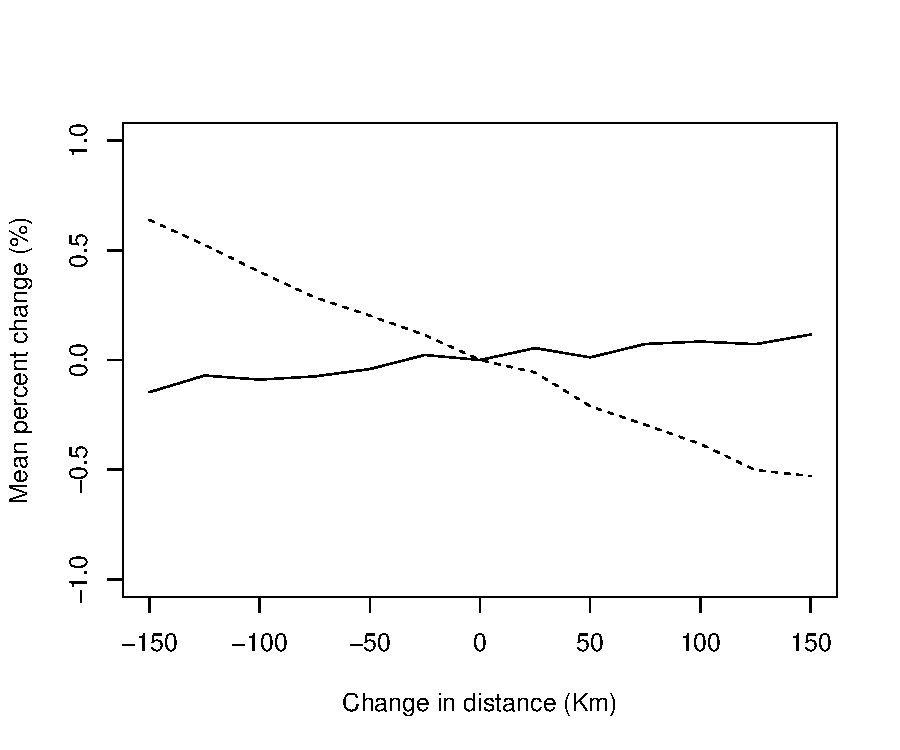
\includegraphics[width=1\linewidth]{fig_distance_modern.pdf}  
%   \caption{}
%   \label{fig:sub-first}

\caption{The effect of decreasing and increasing distance on simulated dental distribution means, averaged across $\xi_j$ and $\xi_a$, for contemporary sand tiger populations. Changes in the juvenile site distributions are denoted by the dashed line; changes in the adult site distributions are denoted by the solid line. In all cases, decreasing or increasing distance $\pm 150 Km$ results in a mean percent difference in distributional means of $<1\%$. 
}
\label{fig:distance}
\end{figure}


\begin{figure}[ht]
  \centering
  % include first image
  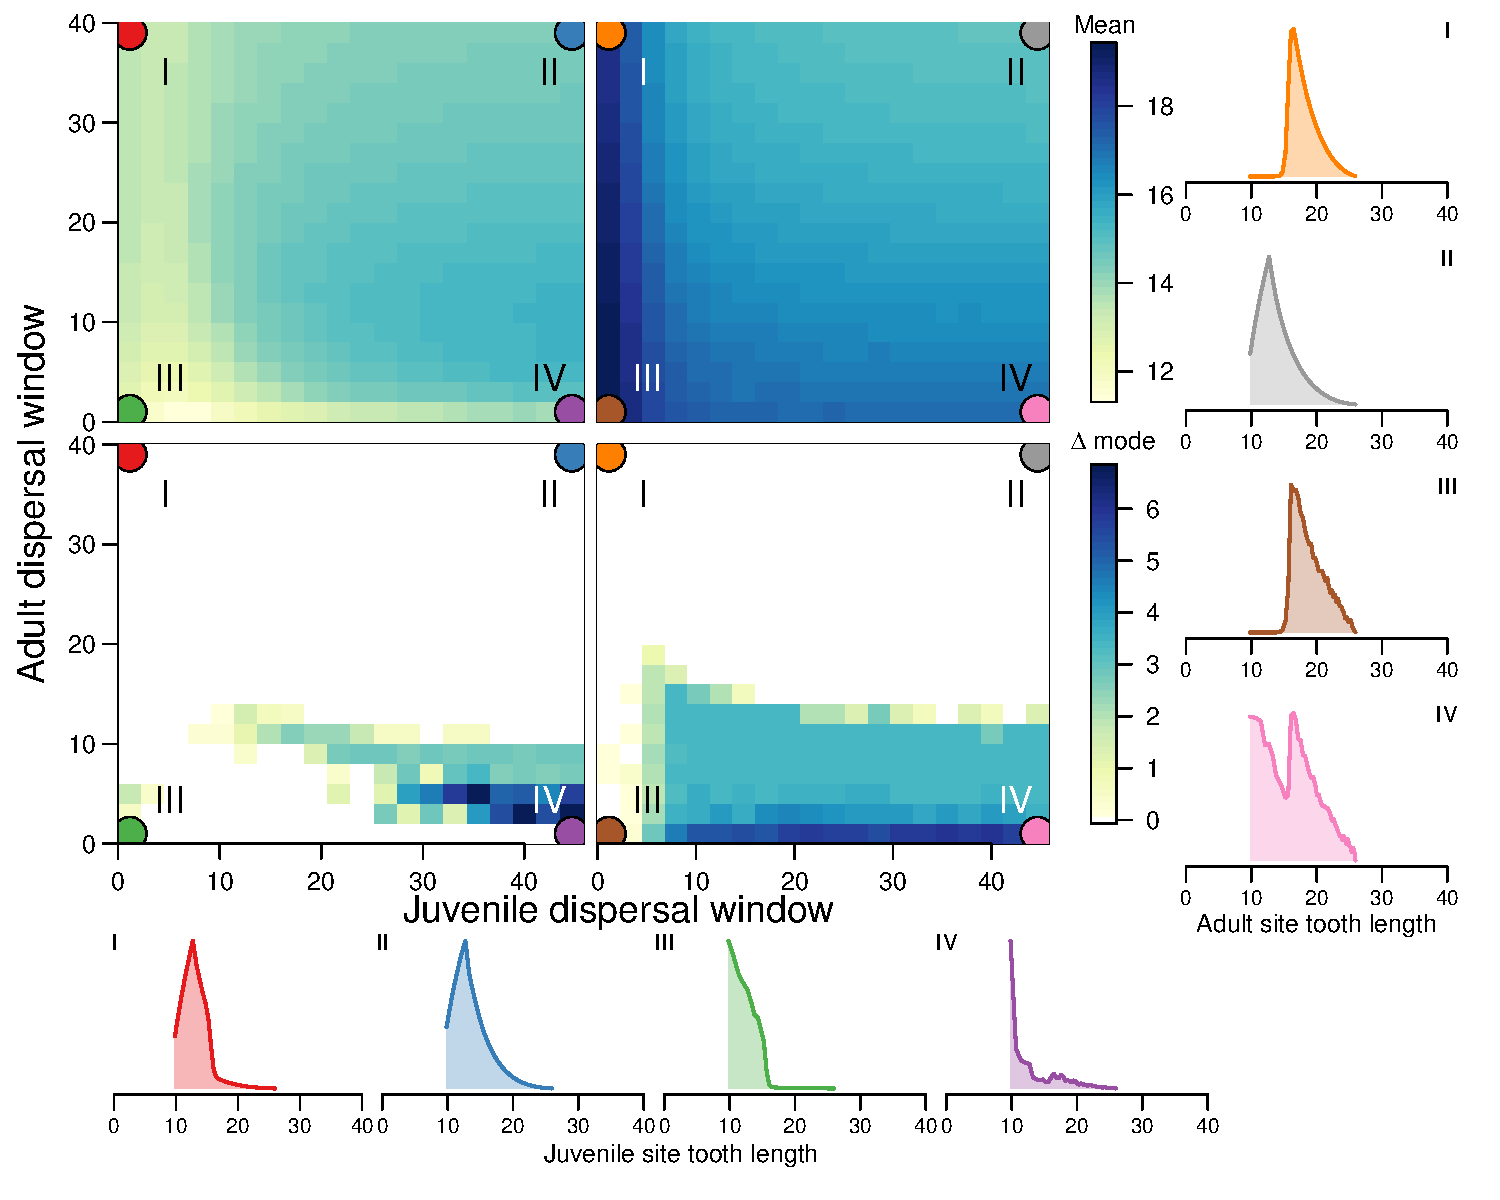
\includegraphics[width=1\linewidth]{fig_means_peaks_modern_rev.pdf}  
%   \caption{}
%   \label{fig:sub-first}

\caption{Simulation results for the dynamic population model as a function of juvenile and adult dispersal windows ($\xi_j$ and $\xi_a$, respectively) given conditions experienced by the contemporary Delaware Bay population. 
Changes in dental distribution shape are captured by site-specific means (top two panels) and the distance between modes ($\Delta$ mode; bottom two panels).
A $\Delta$ mode value of zero means there is only one mode.
% affect the distribution of size, which in turn affects mean anterior tooth crown height (top two panels) as well as presence of multiple modes and distance between these modes (bottom two panels). 
Representative distributions of anterior tooth crown height are shown for juvenile site and adult sites for regions I-IV  (horizontal along bottom and vertical along right edge, respectively), where color denotes both region and site identity.
% The juvenile and adults sites (left vs. right columns) have different distributions of anterior tooth crown height and modes (larger mean sizes and mode differences are shown in darker colors). 
Regions I-IV depict various combinations of small and large dispersal windows. Region I (high $\xi_a$, low $\xi_j$); II (high $\xi_a$, high $\xi_j$); III (low $\xi_a$, low $\xi_j$); IV (low $\xi_a$, high $\xi_j$).
% Results are shown for high altitude Eocene conditions, but are qualitatively similar for all evaluated localities.
% Note the multiple modes that arise when juveniles can leave the nursery across a large body size gradient and adult migration is tightly constrained, as in region IV with size structure for juvenile and adult sites in purple and pink distributions in bottom right.
}
\label{fig:simmodern}
\end{figure}


\begin{figure}[ht]
  \centering
  % include first image
  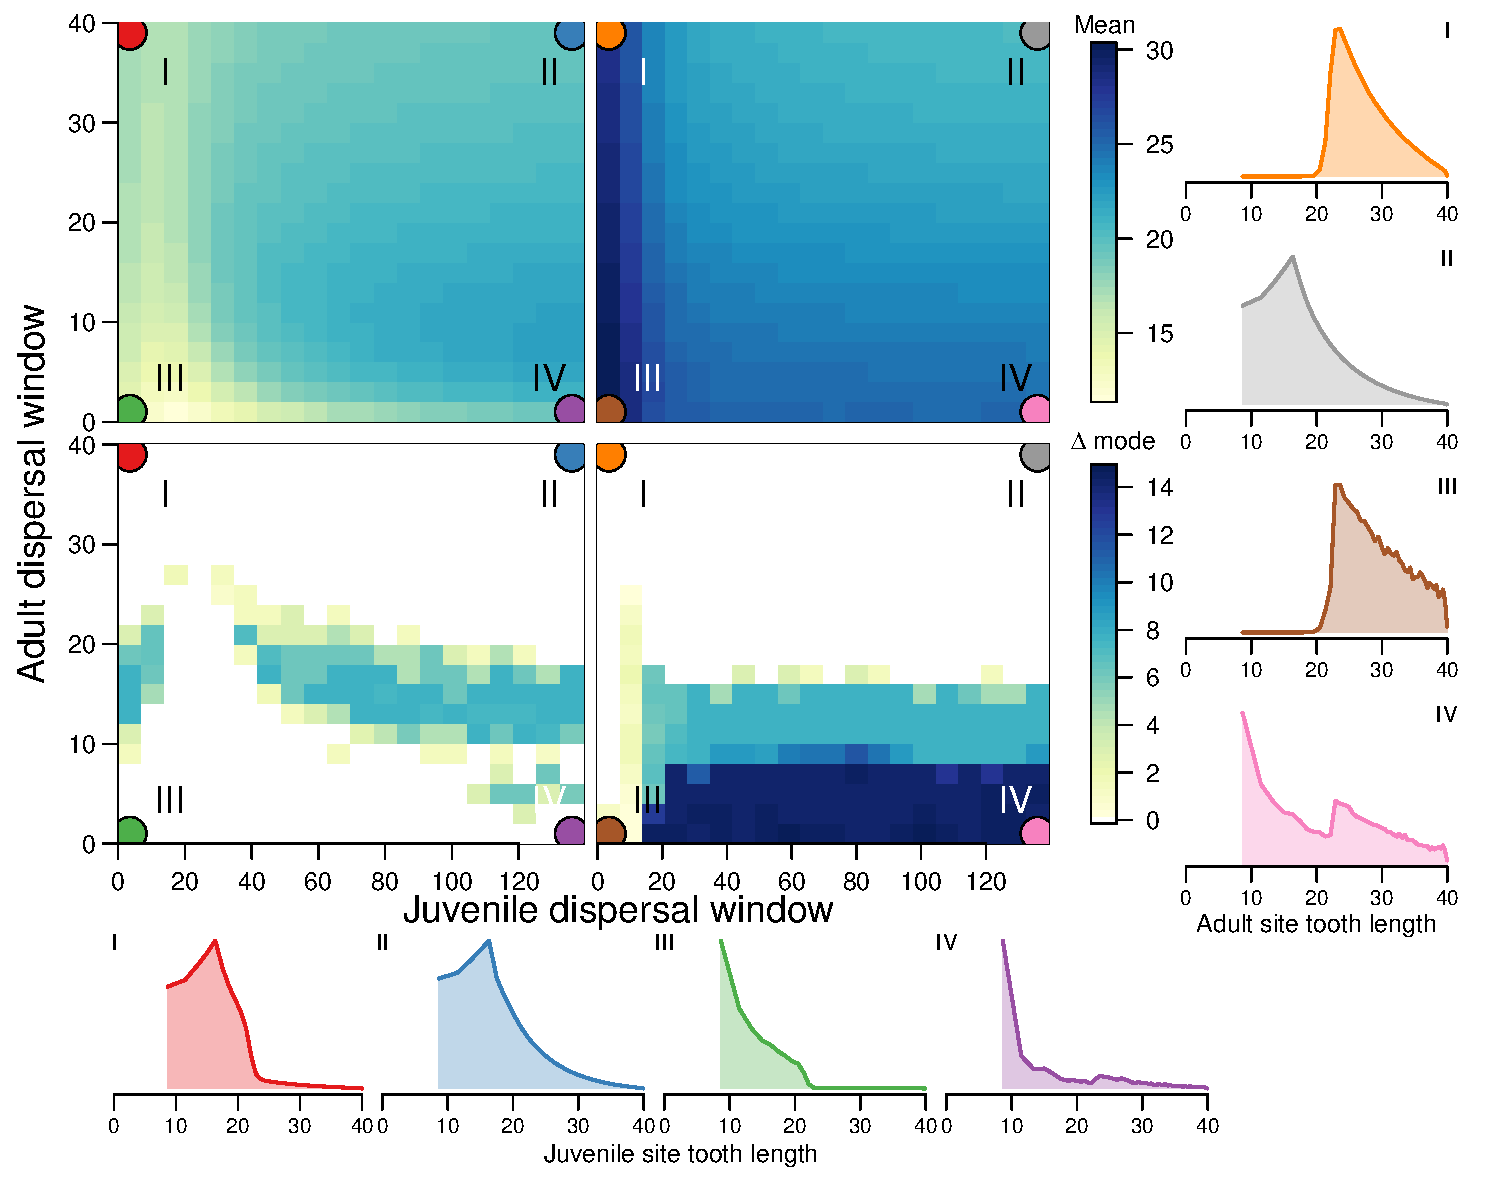
\includegraphics[width=1\linewidth]{fig_means_peaks_eocene_lowlatitude_rev.pdf}  
%   \caption{}
%   \label{fig:sub-first}

\caption{Simulation results for the dynamic population model as a function of juvenile and adult dispersal windows ($\xi_j$ and $\xi_a$, respectively) given low latitude Eocene conditions. 
Changes in dental distribution shape are captured by site-specific means (top two panels) and the distance between modes ($\Delta$ mode; bottom two panels).
A $\Delta$ mode value of zero means there is only one mode.
% affect the distribution of size, which in turn affects mean anterior tooth crown height (top two panels) as well as presence of multiple modes and distance between these modes (bottom two panels). 
Representative distributions of anterior tooth crown height are shown for juvenile site and adult sites for regions I-IV  (horizontal along bottom and vertical along right edge, respectively), where color denotes both region and site identity.
% The juvenile and adults sites (left vs. right columns) have different distributions of anterior tooth crown height and modes (larger mean sizes and mode differences are shown in darker colors). 
Regions I-IV depict various combinations of small and large dispersal windows. Region I (high $\xi_a$, low $\xi_j$); II (high $\xi_a$, high $\xi_j$); III (low $\xi_a$, low $\xi_j$); IV (low $\xi_a$, high $\xi_j$).
% Results are shown for high altitude Eocene conditions, but are qualitatively similar for all evaluated localities.
% Note the multiple modes that arise when juveniles can leave the nursery across a large body size gradient and adult migration is tightly constrained, as in region IV with size structure for juvenile and adult sites in purple and pink distributions in bottom right.
}
\label{fig:simlow}
\end{figure}



\clearpage
%%%%%%%%%% Insert bibliography here %%%%%%%%%%%%%%
\bibliographystyle{RS}
\bibliography{aa_starving3}

% \clearpage
% \section{Supplementary Materials}




\end{document}
